\documentclass{article}
\usepackage{listings}
\usepackage{ctex}
\usepackage{graphicx}
\usepackage[a4paper, body={18cm,22cm}]{geometry}
\usepackage{amsmath,amssymb,amstext,wasysym,enumerate,graphicx,caption,subfigure}
\usepackage{float,abstract,booktabs,indentfirst,amsmath}
\usepackage{array}
\usepackage{booktabs} %调整表格线与上下内容的间隔
\usepackage{multirow}
\usepackage{url}
\usepackage{diagbox}
\renewcommand\arraystretch{1.4}
\usepackage{indentfirst}
\setlength{\parindent}{2em}
\usepackage{listings}
\usepackage{xcolor}
\lstset{
	numbers=left, 
	numberstyle= \tiny, 
	keywordstyle= \color{ blue!70},
	commentstyle= \color{red!50!green!50!blue!50}, 
	frame=shadowbox, % 阴影效果
	rulesepcolor= \color{ red!20!green!20!blue!20} ,
	escapeinside=``, % 英文分号中可写入中文
	xleftmargin=2em,xrightmargin=2em, aboveskip=1em,
	basicstyle=\footnotesize,
	framexleftmargin=2em
} 


\geometry{left=2.8cm,right=2.2cm,top=2.5cm,bottom=2.5cm}
%\geometry{left=3.18cm,right=3.18cm,top=2.54cm,bottom=2.54cm}

\graphicspath{{figures/}}

\title{\heiti 数字电路实验报告 }

\begin{document}
	\vspace*{1cm}
	
	\begin{figure}[h]
		\centering
		
\includegraphics[scale=1.0]{xh.jpg}
	\end{figure}

	\vspace*{0.5cm}
	
	\begin{center}
		\Huge{\textbf{数字电路实验报告}}
	\end{center}
	
	\vspace{5cm}
	
	\begin{table}[h]
		\centering
		\begin{Large}
			\begin{tabular}{p{3cm} p{7cm}<{\centering}}
				实验题目: &   FPGA 原理及 Vivado 综合     \\ \cline{2-2}
				学生姓名:      & 孔浩宇   \\ \cline{2-2}
				学生学号: & PB20000113 \\ \cline{2-2}
				完成日期:       & 2022/11/16 \\ \cline{2-2}
			\end{tabular}
		\end{Large}		
	\end{table}
	\newpage
    \section{实验题目}
        \subsection*{\qquad  FPGA 原理及 Vivado 综合}
     
    \section{实验目的}
        \begin{enumerate}
            \item [1.]了解 FPGA 工作原理
            \item [2.]了解 Verilog 文件和约束文件在 FPGA 开发中的作用
            \item [3.]学会使用 Vivado 进行 FPGA 开发的完整流程
        \end{enumerate}
        
    \section{实验环境}
        \subsection*{\qquad (1) vlab.ustc.edu.cn}
        \subsection*{\qquad (2) fpagol.ustc.edu.cn}
        \subsection*{\qquad (3) Logisim}
        \subsection*{\qquad (4) Vivado}
    
    \vspace*{4cm}
    \section{实验练习}
    \subsection*{题目1} 如图
    \begin{figure*}[htbp]
        \centering
        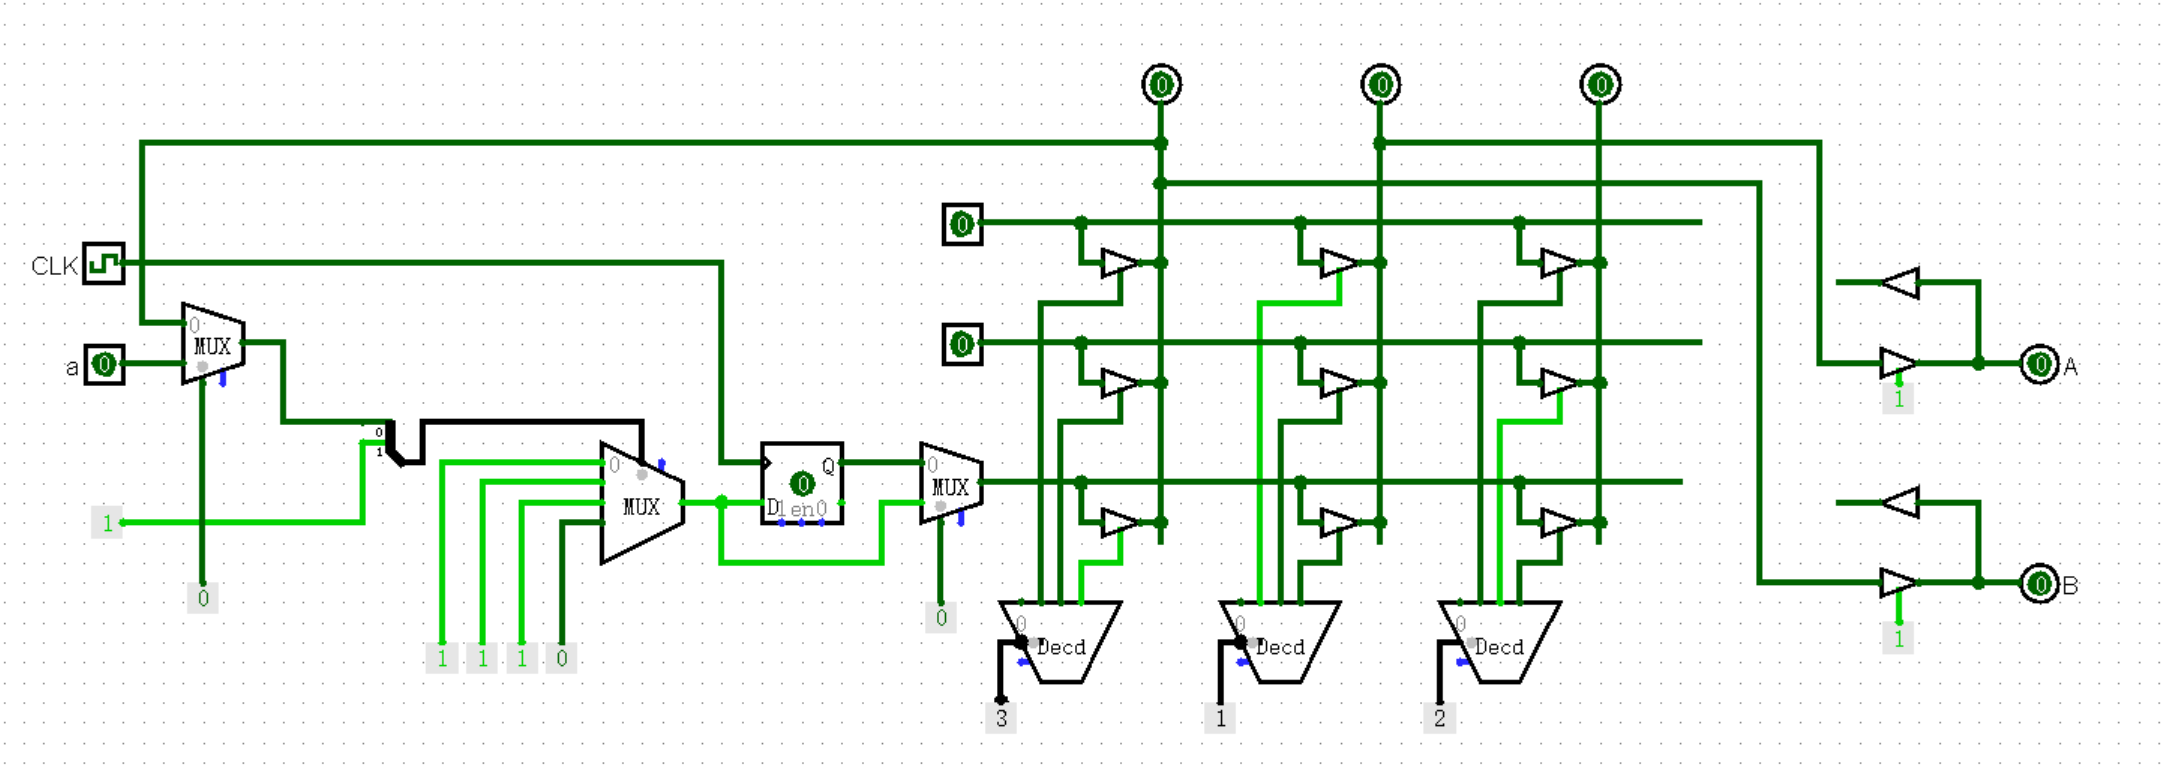
\includegraphics[scale=0.4]{r1.png}
    \end{figure*}
    \clearpage
    \subsection*{题目2} 
    约束文件如图
    \begin{figure*}[htbp]
        \centering
        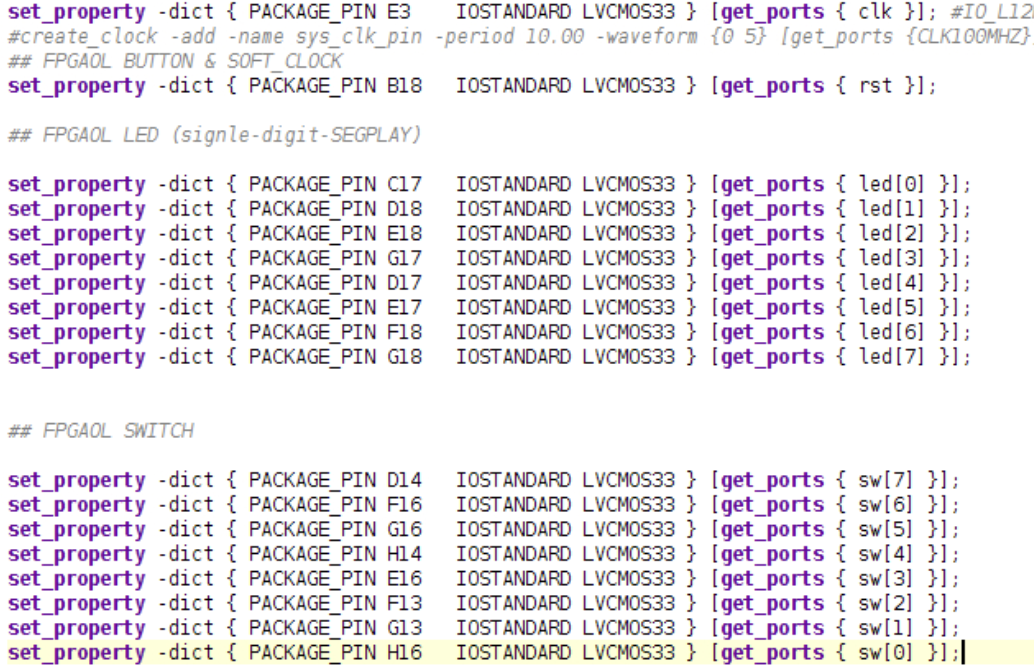
\includegraphics[scale=0.8]{x2.png}
    \end{figure*}

    \vspace*{2cm}
    \subsection*{题目3}
    \begin{enumerate}
        \item [(1)]30位计数器
        
        代码如图
        \begin{figure*}[htbp]
            \centering
            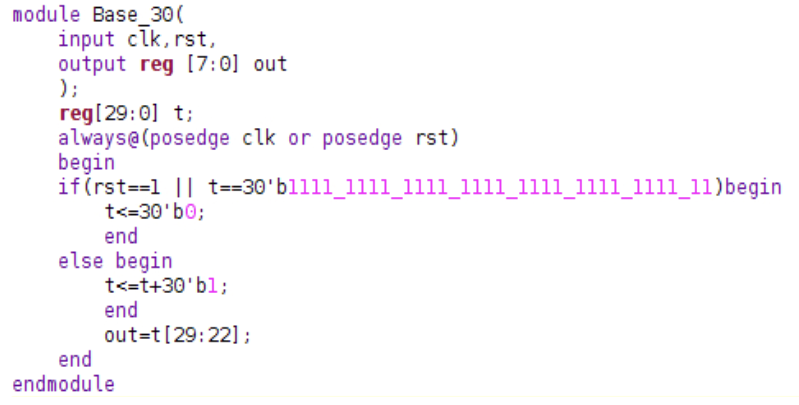
\includegraphics[]{base_30_v}
        \end{figure*}

        \clearpage

        约束文件如图
        \begin{figure*}[htbp]
            \centering
            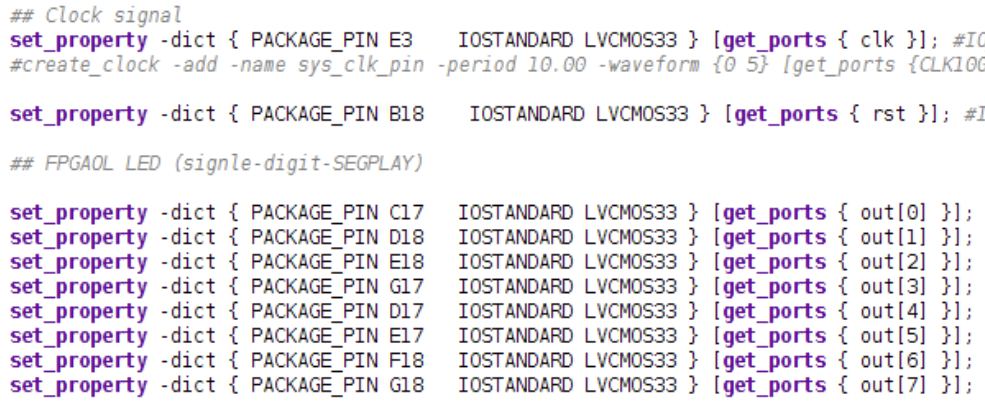
\includegraphics[scale=0.8]{base_30_x}
        \end{figure*}

        结果如图
        \begin{figure*}[htbp]
            \centering
            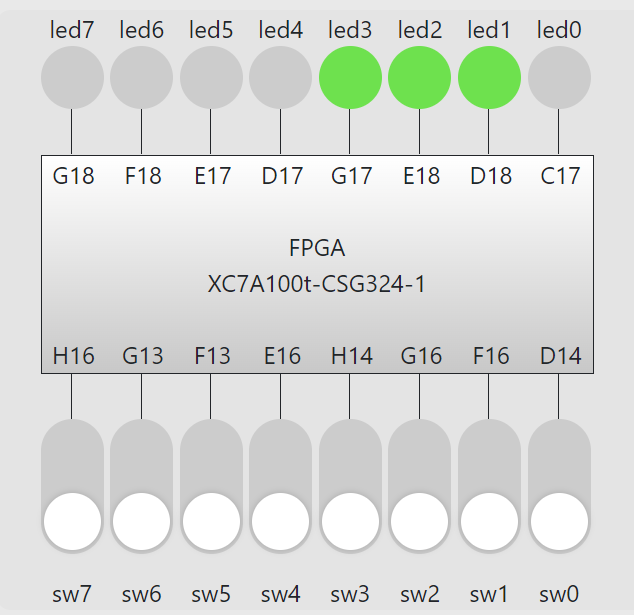
\includegraphics[]{base_30_r}
        \end{figure*}

        \clearpage
        \item [(2)]32位计数器
        
        代码如图
        \begin{figure*}[htbp]
            \centering
            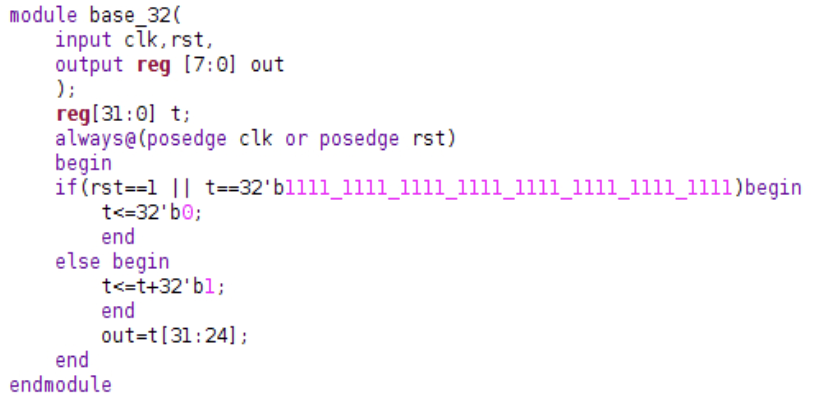
\includegraphics[]{base_32_v}
        \end{figure*}

        约束文件如图
        \begin{figure*}[htbp]
            \centering
            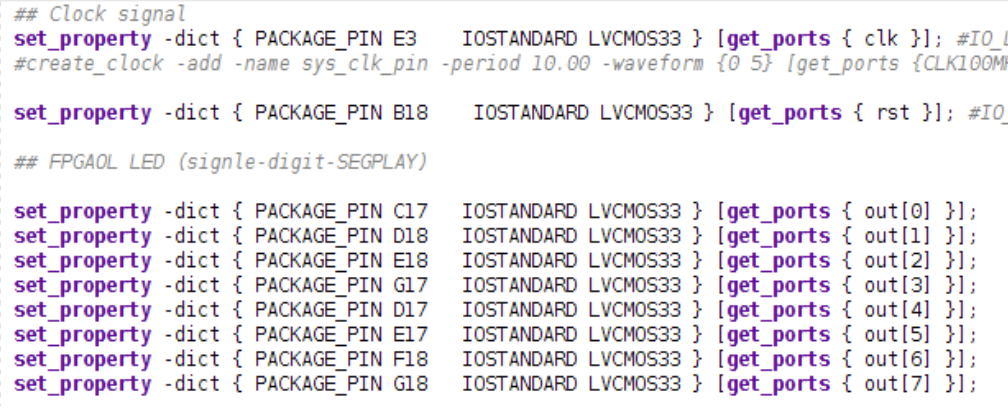
\includegraphics[scale=0.8]{base_32_x}
        \end{figure*}
    \end{enumerate}
	\clearpage
    \section{总结与思考}
	\begin{enumerate}
		\item [1.]学会了用vivado生产bit文件及FPGA烧写
		\item [2.]本次实验难度适中
		\item [3.]本次实验任务量适中
		\item [4.]约束文件可以多给点实例
	\end{enumerate}
\end{document}